\documentclass[11pt,a4j]{jreport}
\usepackage[dvips]{graphicx}
\usepackage{fancybox}
\usepackage{url}
\usepackage{array}
\usepackage{subfig}
\usepackage{color}
\usepackage{listings,jlisting}
\usepackage[dvipdfmx]{hyperref}
\usepackage{pxjahyper}
\lstset{
  %枠外にコードが書かれた時に自動で改行
  breaklines=true,
    %コメントの色
  commentstyle={\itshape \color[cmyk]{1,0.5,1,0}},
  %関数名などの色の設定
  classoffset=0,
  %予約語の色
  keywordstyle={\bfseries \color[cmyk]{0,1,0,0}},
  %枠
  frame=TBrl,
  %行番号とプログラムの間
  framesep=2pt,
  %行が長くなった場合の改行
  breaklines=true,
  %行番号の位置
  numbers=left,
  %行番号の間隔
  stepnumber=1,
  %行番号の書体
  numberstyle=\tiny,
  %空白スペースの記号を出さないようにする
  showstringspaces=false,
  %キャプションの場所
  captionpos=t
}
%hyperrefの設定
\hypersetup{
  setpagesize=false,
  %リンクの色付けをする
  colorlinks=true,
  %目次の文字の色
  linkcolor=black,
  %urlの色
  urlcolor=blue
}
\setlength{\oddsidemargin}{0mm}
\setlength{\textwidth}{170mm} 
\setlength{\topmargin}{-5mm}
\setlength{\textheight}{240mm}
\setlength{\columnsep}{8mm}

%表の水平方向の罫線だけ太くする
\newcommand{\bhline}[1]{\noalign{\hrule height #1}}

\begin {document}
\thispagestyle{empty}
\begin{center}
\begin{Huge}
{\bf 物体認識論 レポート課題}\\
\vspace{0.5cm}
{\bf Web画像を用いた物体認識実験}\\
\vspace{1.5cm}

\begin{tabular}{cc} 
1510161 & 由川 拳都  
\end{tabular}
\end{Huge}
\end{center}

\newpage

\tableofcontents

\chapter{レポート課題1 2クラス画像分類実験}
\section{課題内容}
異なる2クラスの画像をWebAPIによりそれぞれ200枚収集し,2種類の2クラス分類を行った.ポジティブ画像(正例)を図1のようにカレーとし,ネガティブ画像(負例)として寿司とハヤシライスとしてカレーと寿司という似ていない画像での分類,カレーとハヤシライスという似ている画像での分類において様々な分類方法を適用し,分類方法に応じて分類性能がどのように変化するのかを比較した.なお,今回分類方法として
\begin{itemize}
\item カラーヒストグラムとNearest Neighbor法による分類
\item BoFベクトルと非線形SVMによる分類
\item AlexNet,AlexNetに対してConvのカーネル数が減らされた高速ネットワーク

  VGG-16ネットワークによるDCNN特徴と線形SVM,非線形SVMによる分類
\item BoFベクトルと線形SVM,Feature maps法による分類
\item Naive Bayes法による分類
\end{itemize}
の5つの分類方法により2クラス画像の分類を行い,その画像の分類の評価を5分割交差検証(5-fold cross-validation)により行うというプログラムをMATLABにより実装した.なお,Naive Bayes法による分類で5分割交差検証は行っておらず,あくまで参考程度の分類として今回行った.

\begin{figure}[htbp]
  \begin{center}
    \begin{tabular}{c}
      \begin{minipage}{0.35\hsize}
        \begin{center}
    \includegraphics[clip,width=0.5\textwidth]{curry.eps}
        \end{center}
        カレーライス(ポジティブ画像)
      \end{minipage}
      \begin{minipage}{0.35\hsize}
        \begin{center}
          \includegraphics[clip,width=0.5\textwidth]{sushi.eps}
        \end{center}
       \hspace{2.0cm} 寿司

       (似ていないネガティブ画像)
      \end{minipage}
      \begin{minipage}{0.35\hsize}
        \begin{center}
          \includegraphics[clip,width=0.45\textwidth]{hayashi.eps}
        \end{center}
       \hspace{1.7cm} ハヤシライス

        \hspace{0.8cm}(似ているネガティブ画像)
      \end{minipage}
    \end{tabular}
    \caption{実験に用いた画像の一例}
  \end{center}
\end{figure}
\newpage
\section{設計方針}
\subsection{レポート課題1,レポート課題2共通の処理}
まず,以下のURLのように

\url{http://mm.cs.uec.ac.jp/tutorial/flickr.cgi?WORD=&ORDER=2&LOOP=300&THM=1}

予め用意されていたCGIを使ってWeb画像を検索し,画像をダウンロードした.これらの処理をまとめたのがレポート課題1では付録の

\begin{itemize}
\item report1.m
\end{itemize}
であり,レポート課題2では
\begin{itemize}
  \item report2\_prep.m
\end{itemize}
である.

次に,これらの読み込んだ画像をひとつのファイルリストとしてまとめる関数を作成し,このファイルリストの内容をsaveで保存した.
\begin{itemize}
\item filelist.m
\end{itemize}
であり,レポート課題2では
\begin{itemize}
 \item flist.m
 \item flist2.m
\end{itemize}
である

\subsection{レポート課題1での処理}
\begin{itemize}
\item \textbf{カラーヒストグラムとNearest Neighbor法による分類}


読み込んだ画像を引数にしてそれを64色に減色して,正規化させたものを返すmake\_hist.mをまず作成した.次に,5-fold cross validationによる評価を行う際に学習用画像と評価用画像のヒストグラムをを一つのヒストグラムのデータベースとしてまとめ,そのデータベースに対してNearest Neighbor法を適用し,その結果を分類率として返すmファイルreport1\_hist\_nn.mを作成した.\\

\item \textbf{BoFベクトルと非線形SVMによる分類}


はじめにBoFベクトルを生成するために,コードブックの生成を行う関数mk\_codebook.mとBoFベクトルの生成をベクトル化により行う関数mk\_codebook\_vec.mを作成した.

次に,5-fold cross-validationを行うためにポジティブ画像とネガティブ画像のBoFベクトルを学習用と評価用で分けて,それぞれラベル付けを行い非線形SVMによる分類を行う.そして,その正答率を分類率として返すmファイルreport1\_bof.mを作成した.\\

\item \textbf{AlexNet,AlexNetに対してConvのカーネル数が減らされた高速ネットワーク}
  
      \textbf{VGG-16ネットワークによるDCNN特徴と線形SVM,非線形SVMによる分類}
   

AlexNet,高速ネットワーク,VGG-16ネットワークそれぞれによりポジティブ画像とネガティブ画像のDCNN特徴量を格納したリストを5-fold cross-validationでの評価に使うために学習用と評価用で分けて,それぞれラベル付を行い線形SVMと非線形SVMにより分類し,各ネットその正答率を分類率として返すmファイルreport1\_dcnn.mを作成した.\\

\item \textbf{BoFベクトルと線形SVMとFeature maps法による分類}

  
  mk\_codebook.mとmk\_codebook\_vec.mにより作成したポジティブ画像とネガティブ画像が合わさったBoFベクトルに対して5-fold cross validationを行う際に学習用データと評価用データそれぞれにFeature maps法を適用し,適用されたデータに対して線形SVMで分類した時の正答率を分類率として返すmファイルreport1\_featuremap.mを作成した.\\
  
\item \textbf{Naive Bayes法による分類}


まず,正規化処理を行わないで,BoFベクトルを生成したmk\_code\_vec\_nnormal.mという関数を作成し,そのBoFベクトルに対してすべての画像に対して,Naive Bayes法を適用し,その正答率を分類率として返すreport1\_naive.mを作成した.
\end{itemize}

\section{プログラムの説明}

\begin{itemize}
\item \textbf{下準備となるreport1.m,filelist.m}
  
まずreport1.mについて
  
与えられたCGIで検索した画像のURLをリスト化したテキストファイルをMATLABのtextreadで読み込み,それをwebsaveにより画像をダウンロードするという処理を行っているmファイル.

次にfilelist.mについて

カレー(ポジティブ画像),寿司(カレーと分類容易な画像),ハヤシライス(カレーと分類が難しい画像)の各200枚の画像を600枚の一つのファイルリストとして連結し,リストの1〜200番目をカレーの画像,201〜400番目までを寿司の画像と設定し指定画像だけが入ったデータを取り出せるようにし,それを変数に代入することができるようにすることで,実際に分類を行っていくmファイルにおいてリストを使っての処理が簡単になるようにさせるmファイル.
\item \textbf{カラーヒストグラムとNearest Neighbor法による分類}

  \hspace{0.5cm}\textbf{- make\_hist.m report1\_hist\_nn.m}
  
  まず,make\_hist.mについて

  設計方針の項目でも説明をしたが,画像を引数にしてその画像を64色にまで減色して,64次元の画像データになった元の画像に対して関数histcとreshapeによりヒストグラムを作成する.そして,作成されたその正規化させたヒストグラムの値を返すことでヒストグラムインターセクションを求めることができるようにさせている.
\newpage
  次に,report1\_hist\_nn.mについて

  学習用のポジティブ画像とネガティブ画像,そして評価用のポジティブ画像とネガティブ画像を合わせたリストtrainとevalをそれぞれ作成し,それぞれのリストをmake\_histの引数としてヒストグラムを作成するということをtrain,evalの中にある画像の数だけ繰り返す.そして,その結果をそれぞれ学習用画像のヒストグラムのデータベース,評価用画像のデータベースを作り,これらのデータベースを1つのデータセットとして連結して距離行列を作ってNearest Neighbor法を適用する.カレーなら正しくカレーと認識できた割合を分類率としてこれを結果として返す,という処理を5回繰り返し,最終的には5回の分類の平均値を返すというmファイル.また,ヒストグラムインターセクションの類似度が大きいものから順にソートしてそのときの画像をポジティブ画像として認識していると判断してその結果をプロットするという処理も行っている.

\item \textbf{BoFベクトルと非線形SVMによる分類}
  
  \hspace{0.5cm}\textbf{- mk\_codebook.m mk\_code\_vec.m,report1\_bof.m}

  まず,mk\_codebook.mについて

  リストの1〜200番目までをポジティブ画像,201〜600番目までをネガティブ画像としてsift\_rand関数によるdense samplingを行い,sift特徴点を求め,vl\_kmeans関数により1000個の代表的な局所特徴のベクトルの集合(コードブック)を返すmファイル.

  次に,mk\_code\_vec.mについて

  結果を出すということが何よりも優先であると判断したので,確実に正確なBoFベクトルが生成できるように普段の提出課題の模範解答をそのまま利用する形にしたが,説明することにする.
  まずは画像リストのSIFT特徴点を抽出し,128次元のSIFT特徴ベクトルがまとまった行列をコードブックサイズの数だけ縦に複製させた行列とSIFT特徴点の横ベクトルをコードブックの数だけ縦に連続した行列を作り,それぞれの行列の特徴点間の距離を比較しその距離が最小のもの,つまり特徴の類似度が高いものを求めてヒストグラムをつくるという操作を画像の数だけ行うmファイル.


  最後にreport1\_bof.mについて

  学習用のポジティブ画像のBoFベクトルとネガティブ画像のベクトルをtrainという一つのリストに,評価用の画像についても同様にevalという一つのリストにまとめ,学習画像と評価用画像のラベルとなる行列をそれぞれ作り学習画像のリストとそのラベルを使って非線形SVMで学習し,評価データの予測を学習データを使って行い,その正答率(ポジティブ画像を正しくポジティブ画像と認識,ネガティブ画像を正しくネガティブ画像と認識した割合)を返すという操作を5回行い,その平均を最終的な結果とするmファイル.

\item \textbf{AlexNet,AlexNetに対してConvのカーネル数が減らされた高速ネットワーク}

      \textbf{VGG-16ネットワークによるDCNN特徴と線形SVM,非線形SVMによる分類}

      \hspace{0.5cm} \textbf{- report1\_dcnn.m}

      report1\_dcnn.mについて

      各ネットワークでそれぞれポジティブとネガティブ画像合わせて画像600枚の画像を読み込んでFull Connection(fc8)を出力としたDCNN特徴量をリストとしてまとめる.次に,学習用のポジティブ画像のBoFベクトルとネガティブ画像のベクトルをtrainという一つのリストに,評価用の画像についても同様にevalという一つのリストにまとめ,学習画像と評価用画像のラベルとなる行列をそれぞれ作り学習画像のリストとそのラベルを使って線形SVM,非線形SVMそれぞれで学習し,評価データの予測を学習データを使って行い,その分類率を返すという操作を5回行い,その平均を最終的な結果とするという処理を各ネットに対して適用したmファイル.

\item \textbf{BoFベクトルと線形SVMとFeature maps法による分類}

      \hspace{0.5cm} \textbf{- report1\_featuremap.m}

      report1\_featuremap.mについて

      これまでと同様に学習用のポジネガ画像それぞれのBoFベクトルをひとつの学習用画像のリストにし,その次元を3倍に拡張したものを最終的に線形SVMで使う学習用画像のデータセットとした.そして,評価用のポジネガ画像のBoFベクトルも同様にひとつのリストにした後,次元を3倍に拡張し,このデータを学習データをもとにして予測を行うためのデータとして利用している.後は,これまでと同様,分類率を返すという操作を5回繰り返しその平均を最終的な結果とするという処理を行うmファイル.

\item \textbf{Naive Bayes法による分類}

  分類対象の画像を5-fold cross validationで行ってはいないので,あくまで参考程度の分類であるが記していく.

  \hspace{0.5cm} \textbf{- mk\_code\_vec\_nnormal.m, report1\_naive.m}

  mk\_code\_vec\_nnormal.mについて

  Naive Bayes法では識別する際の確率を求めるために学習データのカウント数が必要になる.このため,mk\_code\_vec.mでは行っていた正規化処理をなくしたmファイルがこのファイルで,この処理以外はmk\_code\_vec.mと全く同一である.
  
  report1\_naive.mについて

  すべての画像で学習を行い,すべての画像で分類を行った.具体的には,ポジティブ画像,ネガティブ画像それぞれのBoFベクトルの出現頻度を数え,それを正規化し,対数をとり確率が小さくなりすぎるということを防ぐという処置をとったあと,未知画像に対してそれがポジティブ画像である確率とネガティブ画像である確率を求める.その結果の正答率を分類率として返すというNaive Bayes法の一連の処理を記述したmファイル.
\end{itemize}


\section{実験}
収集を行ったデータはまず,カレーが\url{http://mm.cs.uec.ac.jp/tutorial/flickr.cgi?WORD=curry&ORDER=4&LOOP=200&THM=1}のようにkeywordをcurry,orderをrelevanceとした画像200枚を収集した.次に,寿司は\url{http://mm.cs.uec.ac.jp/tutorial/flickr.cgi?WORD=sushi&ORDER=4&LOOP=200&THM=1}のようにkeywordをsushi,orderをrelevanceとして画像を200枚収集した.そして,ハヤシライスはのようにkeywordを日本語でハヤシライス,orderをrelevanceとして200枚の画像を収集した.(なお,検索結果のURLは\LaTeX のhyperrefでは日本語では検索結果が文字化けしてしまい,正しく出なかったのでURLは示さない.)

なお,ハヤシライスについて自分がよく確認をしなかったという自分の落ち度で収集した画像の中で15枚のハヤシライス(ルーも含めて)全く写っていない画像を収集してしまっている.


各分類方法によるカレー/寿司,カレー/ハヤシライスの2クラス画像分類の結果は以下の通り.
\begin{table}[htb]
  \begin{center}
    \caption{各分類方法による分類率の結果}
    \begin{tabular}{ccc}  \bhline{2pt}
      分類方法 & 分類率(カレーと寿司) & 分類率(カレーとハヤシライス)\\ \hline
      カラーヒストグラム+NN法 & 77.3\% & 82.8\% \\
      BoF+非線形SVM &  89.5\%  & 75.5\%  \\
      BoF+線形SVM+Feature maps法 &  91.25\% & 79.25 \% \\ 
      Naive Bayes法(参考記録) &  91.5\% &  61.5\% \\ \bhline{2pt}
    \end{tabular}
  \end{center}
\end{table}
\newpage
\begin{table}[htb]
  \begin{center}
    \caption{各分類方法による分類率の結果(DCNN特徴量+SVM)}
    \begin{tabular}{ccc}  \bhline{2pt}
      分類方法 & 分類率(カレーと寿司) & 分類率(カレーとハヤシライス)  \\ \hline
      AlexNetによるDCNN特徴と線形SVM &  99.5\% & 90.0\% \\
      AlexNetによるDCNN特徴と非線形SVM &  99.0\%  & 91.75\%  \\
      高速ネットによるDCNN特徴と線形SVM &  99.75\% & 91.0\% \\
      高速ネットによるDCNN特徴と非線形SVM &  99.75\% & 93.0\% \\
      VGG-16ネットによるDCNN特徴と線形SVM &  99.75\%  & 91.75\%  \\
      VGG-16ネットによるDCNN特徴と非線形SVM & 99.75\% & 93.25\% \\ \bhline{2pt}
    \end{tabular}
 \end{center}
\end{table}


認識結果の画像の例はうまく分類結果を示すことができたカラーヒストグラムとNearest Neighbor法による分類を行った時の分類結果の画像のみを示す.

\begin{figure}[htbp]
  \begin{center}
    \begin{tabular}{c}
      \begin{minipage}{0.5\hsize}
        \begin{center}
          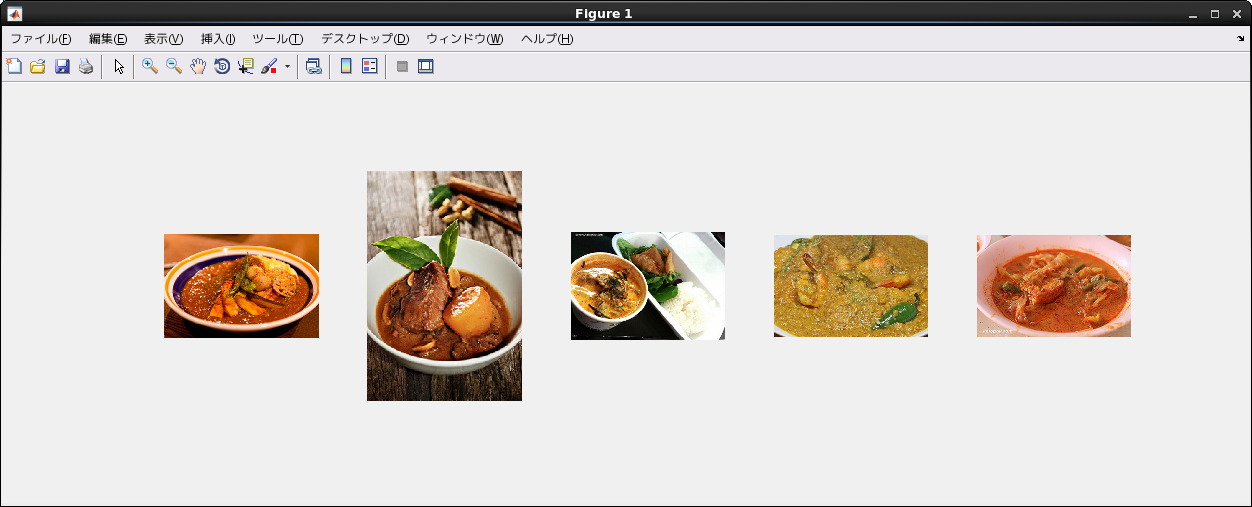
\includegraphics[clip,width=0.95\textwidth]{sushi_hist.eps}
        \end{center}
        \hspace{2.2cm}カレーと寿司の場合
      \end{minipage}
      \begin{minipage}{0.5\hsize}
        \begin{center}
          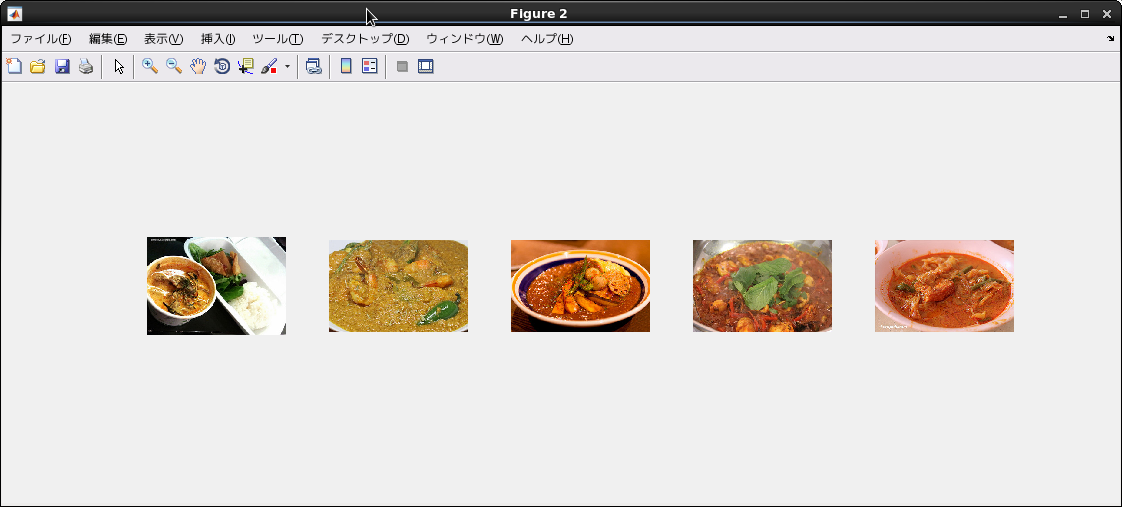
\includegraphics[clip,width=0.95\textwidth]{hayashi_hist.eps}
        \end{center}
        \hspace{2.2cm}カレーとハヤシライスの場合
      \end{minipage}
    \end{tabular}
    \caption{カラーヒストグラムとNearest Neighbor方による分類結果の一例}
  \end{center}
\end{figure}
\newpage
Flickrにより検索した元画像と今回の結果を照らしあわせてみると,いずれもカレーの画像であったため,ヒストグラムインターセクションを求めたことにより表示した画像の一例は正しく認識できていると判断した.

\section{考察}

まずは,今回の分類結果の妥当性を検証してみることにする.表1.1,表1.2をみてみると,ヒストグラムとNearest Neighbor法による分類以外はカレーと寿司との分類率がカレーとハヤシライスの識別率を上回るという結果になった.カレーとハヤシライスの2クラス分類を似ていない画像どうしの分類と設定したので,のこの分類率のほうが低かったということは画像を認識し,識別するという操作を適切に行っているからこそ算出された結果であると考えられるので,妥当性のあるものであると考える.ヒストグラムとNearest Neighbor法による分類でのみカレーとハヤシライスの分類のほうが分類率が高い理由は単純に,カレーとハヤシライスの色(ごはんや具の色)が寿司と比較した場合に比べて似ているためであると考える.これは,2クラス間の色のヒストグラムの類似度が近いものを抽出するという操作をこの分類では行っているため当然といえば,当然の結果であると言える.\\

次に,BoFベクトルと非線形SVMによる分類とBoFベクトルと線形SVM,Featuremaps法による分類結果について考えてみることにする.表1.1の結果を見るとBoF+非線形SVMの分類よりもBoF+線形SVM+Feature maps法の分類率のほうが高いという結果になった.今回,それぞれの実行時間を計測することを失念していたため,Feature maps法での高速化の検証は行うことができなかったが,少なくともこの結果からFeature maps法で学習データと評価データを高次元のものへと写像するという処理をあえて行うことで,非線形SVMを使うことで出していた非線形な決定境界の決定という問題から線形分離可能な境界を引くという計算が簡単な問題に帰結することができたため線形SVMで分析を行っても精度が非線形分離を行った場合と遜色ない,今回の場合は改善が見られたという原理の裏付けを行うことができていると考える.
この方法が深層学習による分類結果を除けば5-fold cross validationを行って,学習データや評価データを一様にしているにも関わらず最も高い分類率を示していた.この結果から,SVMは分析性能がいいが計算が遅いというよく聞くような文言も,このように近似的な写像関数をつくり,高次の次元への写像を行うというお膳立てを使ってあげると計算の遅さを気にすることなく解決ができているといえ、この強みが講義で紹介されていたようにSVMを有名にさせたという考えは支持のできるものであると考える.\\

最後に,表1.2のDCNN特徴とSVMによる分類率の結果について考えることにする.まず結果の比較がしやすいカレーとハヤシライスの似ていない画像どうしの分類結果をみると,最も正確に分類しているのはVGG-16ネットと非線形SVMの結果が最も高い分類率を示していて,AlexNetと線形SVMの分類のほうが最も低い分類率であった.これらの識別率から考えてみるとは実験結果は原理の裏付けとなっているといえるので妥当性があるものとして考える.カレーとハヤシライスの分類率のほうが低かったのは,DCNN特徴で持ってしてもカレーとハヤシライスではご飯や具などの形状や色が似ているためカレーとハヤシライスを説明するのに最たる特徴が寿司に比べると抽出が困難であったためであると考える.
\newpage
\section{感想}
レポートで考察を書くためにいろいろ復習をしていて,分類は行いはしたので参考程度として掲載したNaive Bayes法の分類において,5-fold cross validationを使った方法の方針が思い浮かんでしまうなど,プログラムを色々と見返してみるとミスが少なからず見受けられてしまった実験であり,また提出優先で愚直なコードを書いてしまった部分もあり,リファクタリングができなかったことも自分としては心残りである.
IEDの利用期間が今年の場合は制約がかかっていたので先に先にと早めに取り掛っておけば,自分でも満足のいく内容をこの課題に対してレポートとして残すことができたのになぁと悔やんだ実験であった.

また,考察を行うために講義で紹介されていたことを書籍やWebサイトで調べ直すということを行ったので,レポートを機会に復習を行うことができ,Naive Bayes法とFeature maps法,カーネルトリックといった多次元への写像を使った分類処理の原理の理解を深められたことが自分にとってこの実験の一番の収穫である.
しかしながら,講義を聞いていた時も実際にプログラムを書いている時も思っていたのだが,BoFベクトルの作り方に関する話題は未だになんとなくやろうとしていることが分かる程度の理解しかないので,今後,4年生以降で研究室でこの手の機械学習の手法や深層学習の手法とは長い付き合いになる予定でいるので,この物体認識論という科目だけの話題として終わらせるのではなく,データの学習手法の1つのアプローチとして理解を深める必要があると感じさせる実験だった.

余談ではあるが,このような画像認識実験を行うことで深層学習でのCNNを使っての特徴抽出の精度の高さと計算時間のかかり具合(report1\_dcnn.mの結果が出るまでに10分程度かかった.)を思い知った.(実験中最も時間がかかったのはコードブックとBoFベクトルの生成ではあったが)

\chapter{レポート課題2 Web画像検索リランキング実験}

\section{課題内容}
レポート課題1で行っていたFlickrによる画像収集をある特定の2つのキーワード(今回はコンピュータと目玉焼き)の検索結果300枚に対して行い,そのうち\textit{n}=25枚もしくは50枚を間違いが含まれていても気にすることなくポジティブポジティブ学習画像とし,ネガティブ学習画像を/usr/local/class/object/bgimgにあるランダム画像1000枚とした.

そして,学習画像すべてからAlexNetによるDCNN特徴量を抽出し,残りの\textit{n+1}〜300枚までを評価画像として線形SVMによる分類を行い,その出力結果のスコアからもとのFlickrの画像検索の結果上位100枚リランキングを行った結果上位100枚との認識精度の比較を行った.
\begin{figure}[htbp]
\begin{center}
  \begin{tabular}{c}
    \begin{minipage}{0.35\hsize}
      \begin{center}
        \includegraphics[clip,width=0.5\textwidth]{computer.eps}
      \end{center}
      \hspace{1.5cm}コンピュータ
    \end{minipage}
    \begin{minipage}{0.35\hsize}
      \begin{center}
        \includegraphics[clip,width=0.5\textwidth]{medama.eps}
      \end{center}
     \hspace{2.2cm}目玉焼き
    \end{minipage}
  \end{tabular}
  \caption{実験に用いた画像の一例}
\end{center}
\end{figure}

\section{設計方針}
はじめに,下準備に関しては1.2.1で記した通りの方針で行った.

次に,ポジティブ画像とネガティブ画像のリストを学習用と評価用に分けそれぞれDCNN特徴量を抽出し,線形SVMで学習用画像を学習し,評価用データをその学習用画像でラベルを予測する.そして,その結果の出力スコアを降順にソートするという操作を行った.その結果を画像名とそのURLとスコアをコンソール表示する.この処理を行っているのがreport2.mである.

このreport2.mによって出された画像URLをテキストファイル形式で保存し,予め用意されていた画像をファイル名順に出力するPerlでのHTML生成スクリプトによりHTMLファイルを生成し,そのHTMLファイルをブラウザ上で見て結果を確認し,このうち上位100枚のリランキング結果を元画像であるFlickrの検索結果上位100枚と自分で基準を設けて,正しくコンピュータや目玉焼きだと認識できている画像を数えることでリランキング性能の比較を行った.

\section{プログラムの説明}
\begin{itemize}
\item \textbf{report2\_prep.m}

  report1.mと全く同一の内容を行うもので,与えられたCGIで検索した画像のURLをリスト化したテキストファイルをMATLABのtextreadで読み込み,それをwebsaveにより画像をダウンロードするという処理を行っているmファイル. 
\item \textbf{flist.m,flist2.m}

  flist.mはコンピュータの画像と(ポジティブ画像),ランダム画像(ネガティブ画像)をひとつのファイルリストとして連結させ,実際に分類を行っていくmファイルにおいてリストを使っての処理が簡単になるようにさせるmファイル.

  flist2.mはポジティブ画像を目玉焼きとしただけで残りはflist.mと同一である.
\item \textbf{report2.m}
  
1〜\textit{n}(25or50)枚までのポジティブ画像とランダム画像であるネガティブ画像を合わせて1つの学習用画像リストとして作成し,残りのポジティブ画像である\textit{n+1}〜300枚までの画像とランダム画像であるネガティブ画像を一つの評価用画像リストとする.それぞれに対してDCNN特徴量を抽出しする.そして,抽出した学習用画像のDCNN特徴量のリストで学習ラベル作り,DCNN特徴量による学習データとラベルにより線形SVMで学習を行う.その学習した結果を評価用画像のDCNN特徴量に対する予測で利用し,その分類結果の信頼度が大きいものを降順にソートして,その結果として画像名とスコアをコンソール上に出力するmファイル.
\end{itemize}

\section{実験}

キーワード「コンピュータ」に関して\url{http://mm.cs.uec.ac.jp/tutorial/flickr.cgi?WORD=computer&ORDER=2&LOOP=300&THM=1}のようにkeywordを「computer」,orderを「interesting」,画像を300枚で検索し,その検索結果をノイズを気にすることなくそのまま収集した.キーワード「目玉焼き」に関してはkeywordを日本語で「目玉焼き」,orderを「relevance」,画像を300枚で検索し,その検索結果をノイズを気にすることなくそのまま収集した.(URLは1.4節でハヤシライスの箇所で説明したように日本語で検索を行ったため今回は示さない.)

検索したキーワード「computer」と「目玉焼きの」flickrの元画像100枚とn=25,50とした時のリランキング結果の一部をそれぞれ以下の図に示す.
\newpage
\begin{figure}[htbp]
  \begin{center}
          \includegraphics[clip,width=\textwidth]{flickr_com100.eps}
        \caption{Flickrの元画像上位100枚(キーワード:computer)}
  \end{center}
\end{figure}
  

\begin{figure}[htbp]
  \begin{center}
    \begin{tabular}{c}
      \begin{minipage}{0.5\hsize}
        \begin{center}
          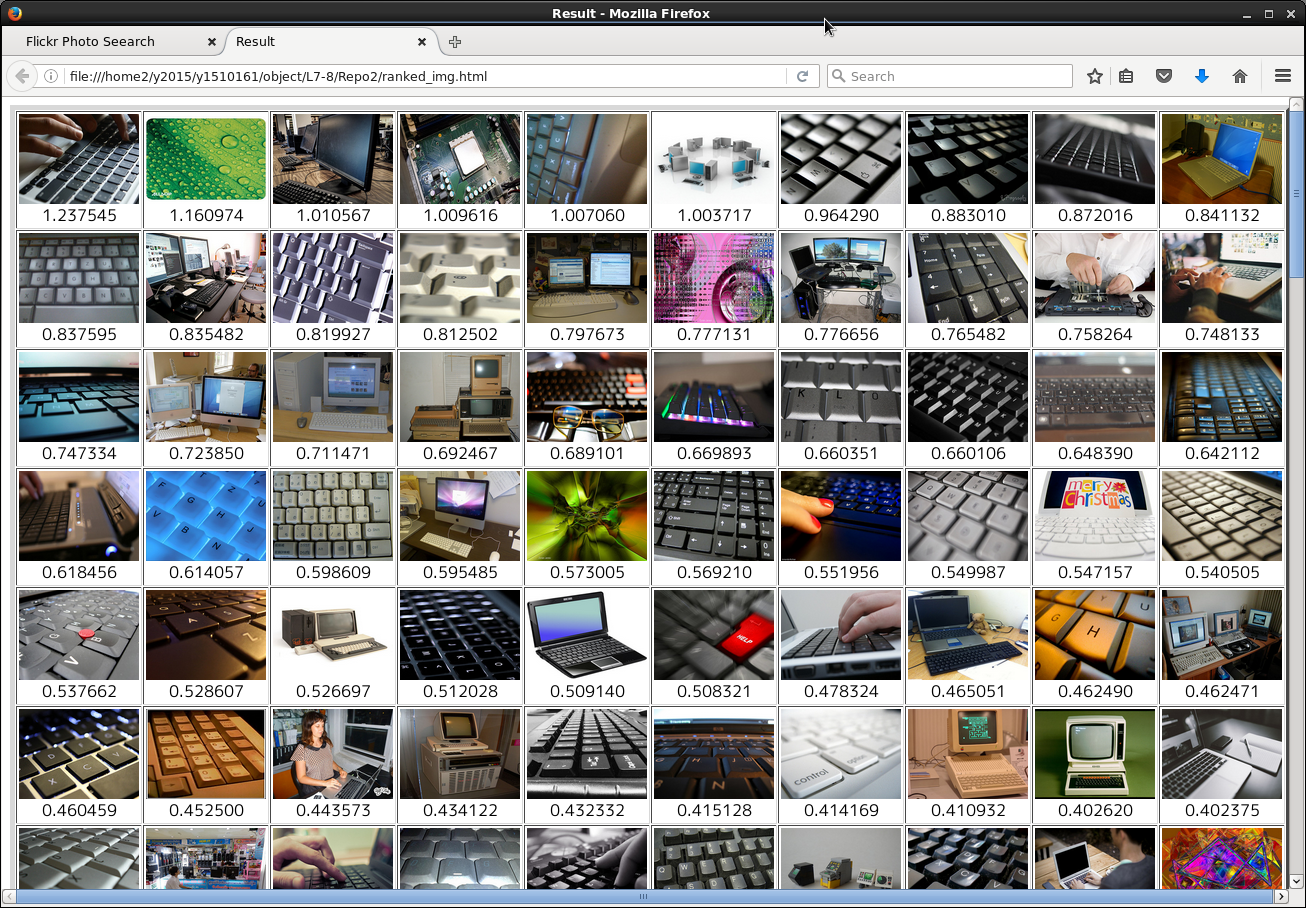
\includegraphics[clip,width=\textwidth]{rankresult_25.eps}
        \end{center}
        \hspace{3cm} \textit{n}=25の時
      \end{minipage}
      \begin{minipage}{0.5\hsize}
        \begin{center}
          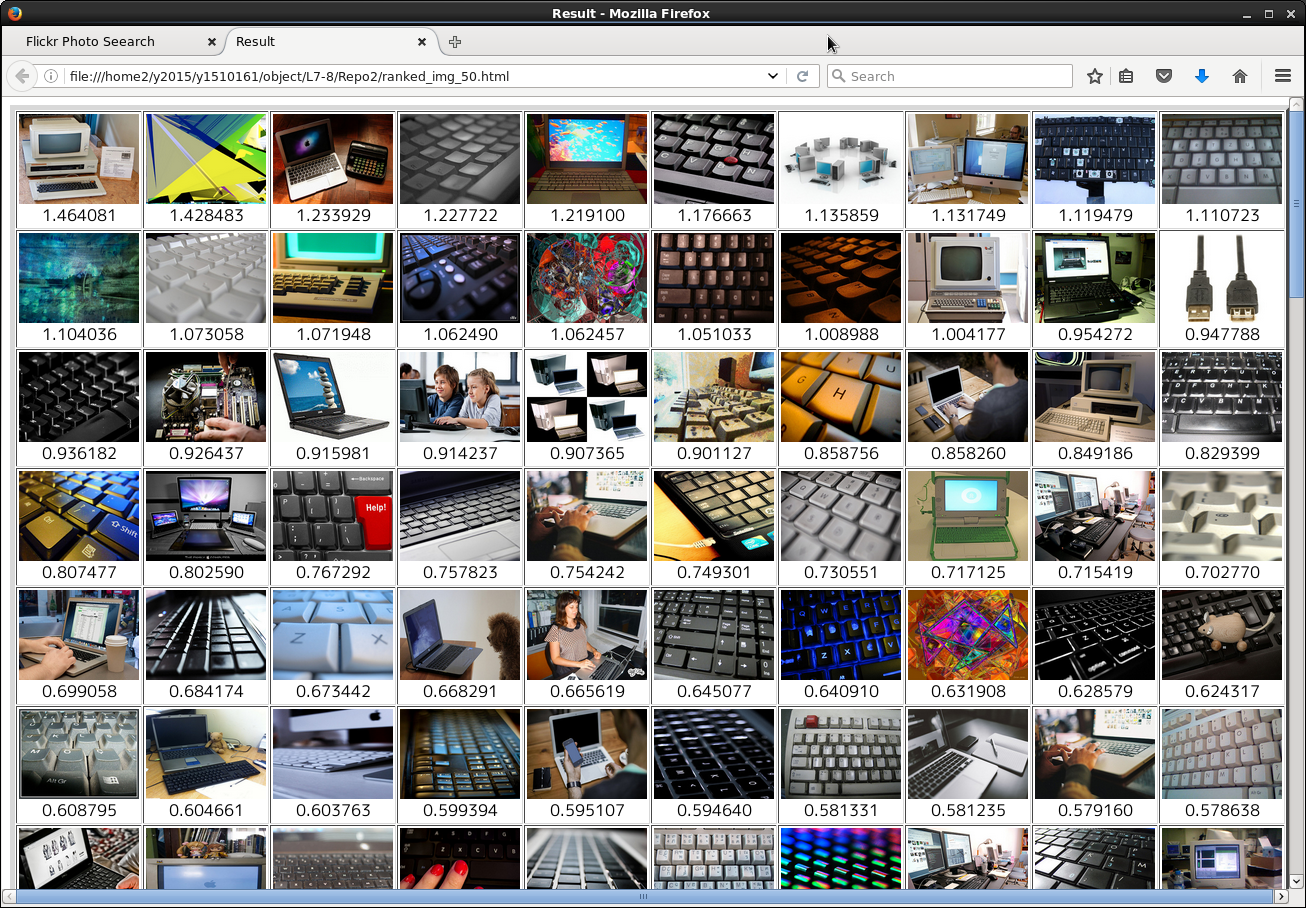
\includegraphics[clip,width=\textwidth]{rankresult_50.eps}
        \end{center}
        \hspace{3cm}\textit{n}=50の時
      \end{minipage}
    \end{tabular}
    \caption{キーワード:computer \textit{n}=25,\textit{n}=50のときのリランキング結果の一部}
  \end{center}
\end{figure}

\newpage
\begin{figure}[htbp]
    \begin{center}
      \includegraphics[clip,width=\textwidth]{flickr_medama_100.eps}
      \caption{Flickrの元画像上位100枚(キーワード:目玉焼き)}
    \end{center}
  \end{figure}

  \begin{figure}[htbp]
    \begin{center}
      \begin{tabular}{c}
        \begin{minipage}{0.5\hsize}
          \begin{center}
            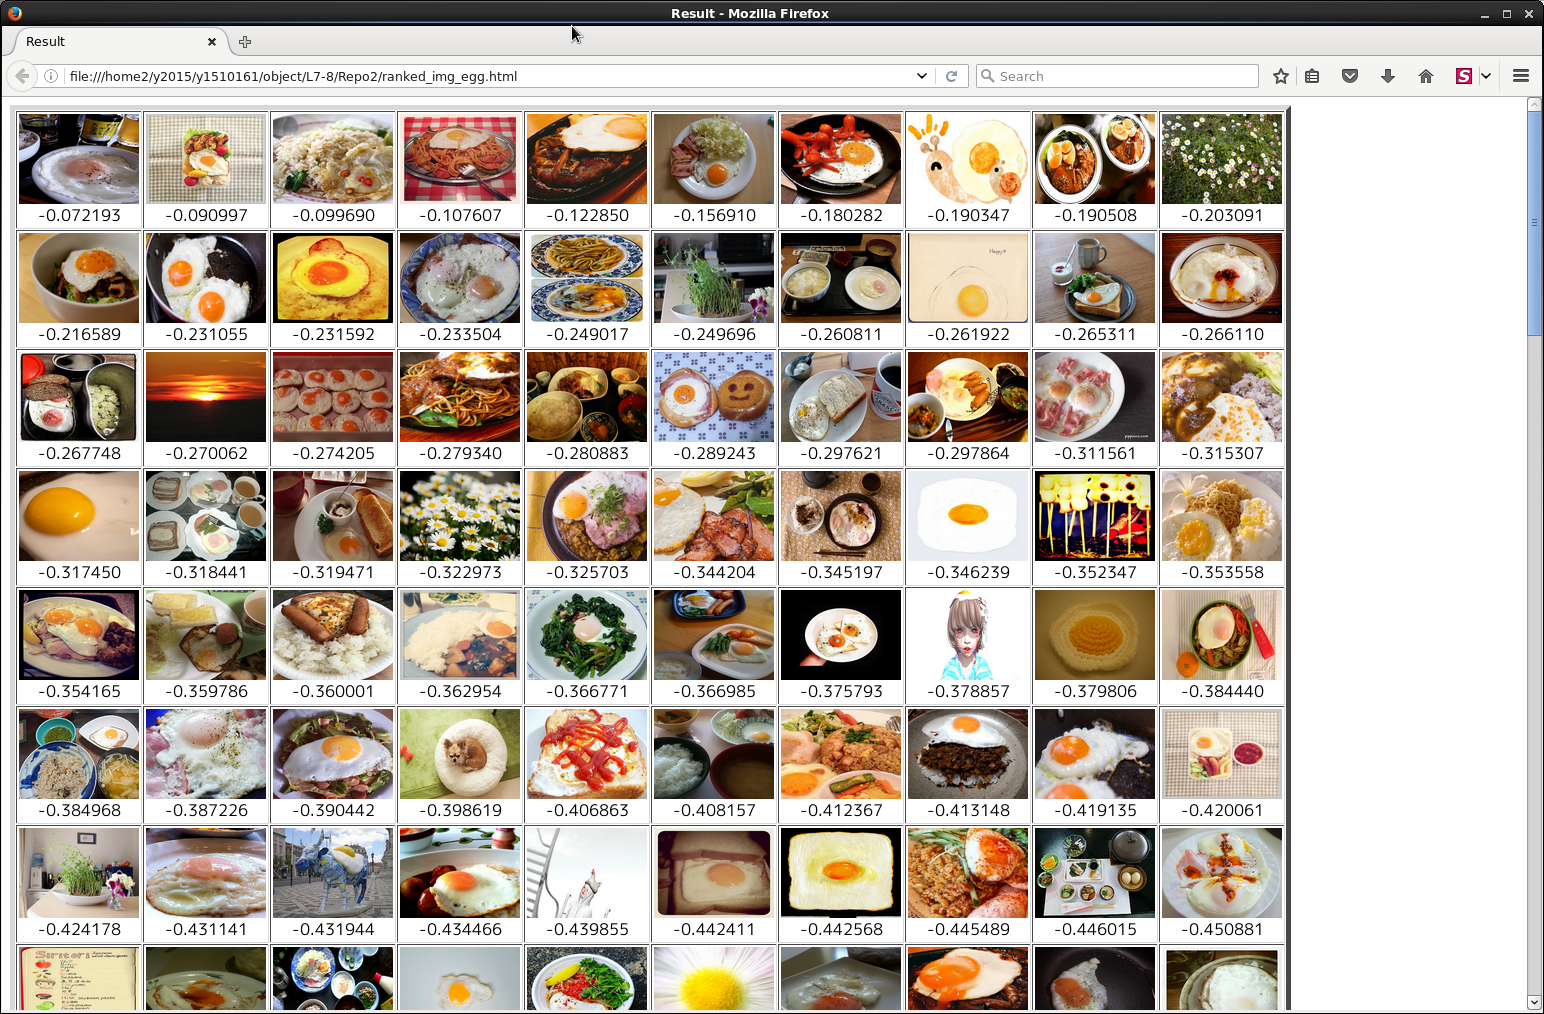
\includegraphics[clip,width=\textwidth]{ranked_egg_25.eps}
          \end{center}
          \hspace{3cm} \textit{n}=25の時
        \end{minipage}
        \begin{minipage}{0.5\hsize}
          \begin{center}
            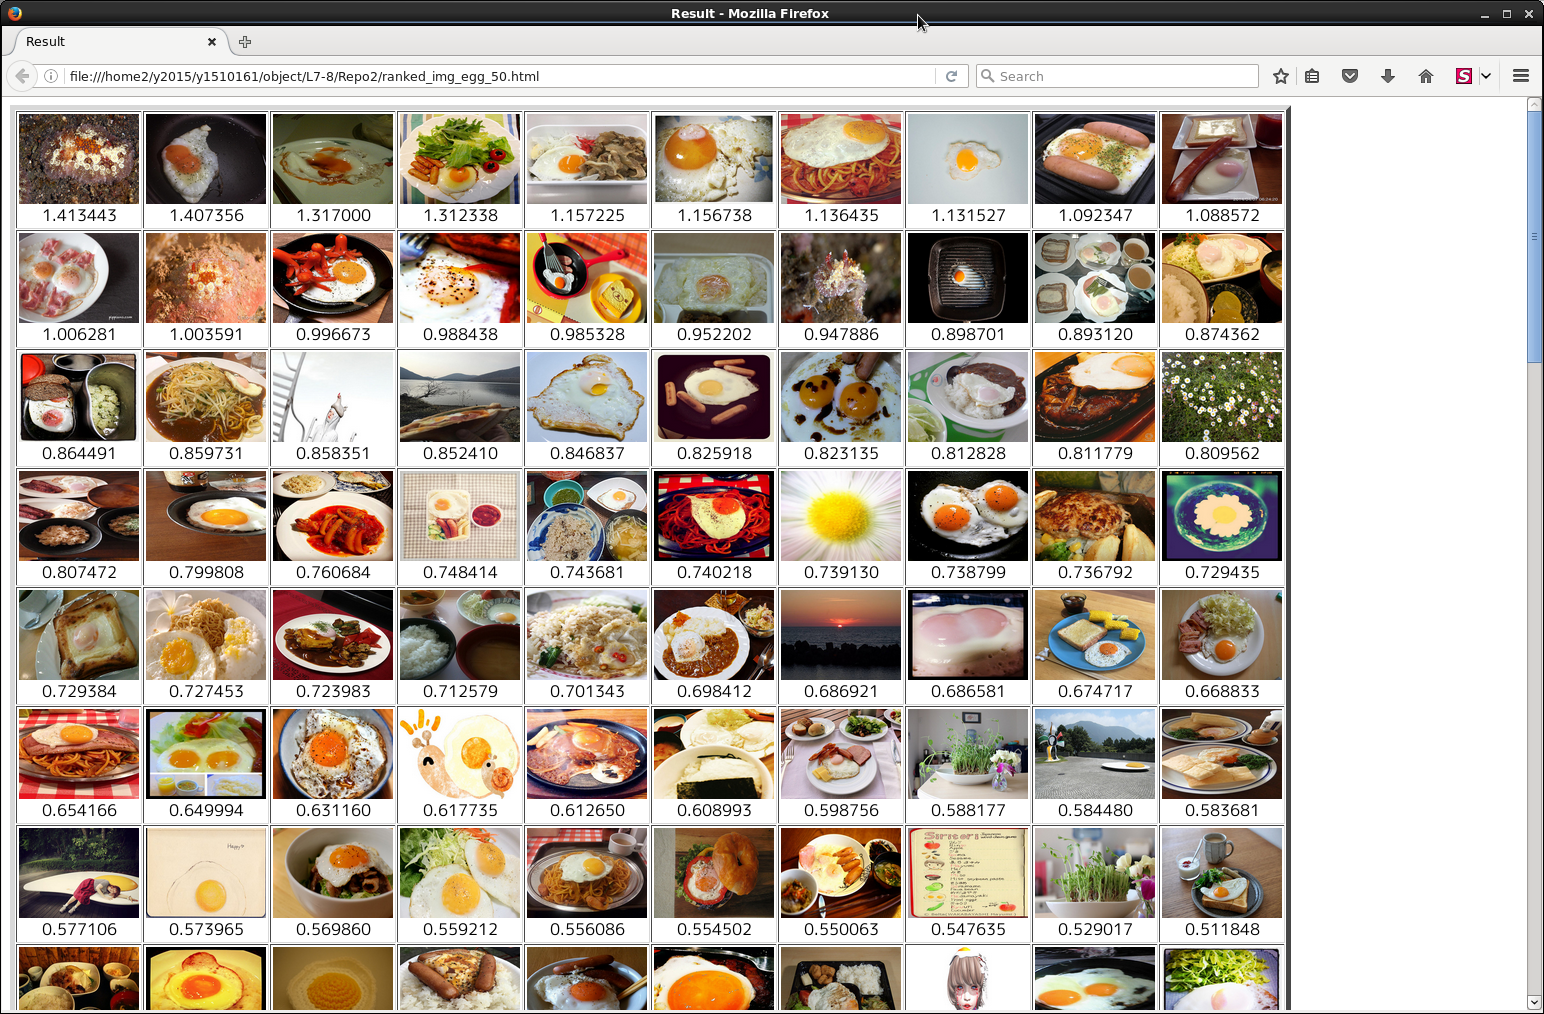
\includegraphics[clip,width=\textwidth]{ranked_egg_50.eps}
          \end{center}
          \hspace{3.3cm}\textit{n}=50の時
        \end{minipage}
      \end{tabular}
      \caption{キーワード: 目玉焼き \textit{n}=25,\textit{n}=50のときのリランキング結果の一部}
    \end{center}
    \end{figure}

  この結果を見てリランキング性能を元画像上位100枚と\textit{n}=25,50の時のリランキング結果上位100枚の結果とを自分で基準を設けて比較した.2つのキーワード「computer」と「目玉焼き」それぞれの基準は以下の通りにした.
\begin{itemize}
  \item キーワード「computer」
    \begin{itemize}  
    \item  元画像がキーボードが多かったため,キーボードもコンピュータの一部であると考えて正解とした.
    \item  ノートPCであれデスクトップ型であれコンピュータであると判断し,人が写っている画像でもコンピュータが写っていれば正解とした
    \item  回路素子などはコンピュータの構成要素ではあるのだが,あくまでもコンピュータの外見では見えるものではないので不正解とした.
    \item 明らかにコンピュータでないもの(今回,幾何学模様が見受けられた)は不正解とした.
     \end{itemize}
\end{itemize} 
\newpage
\begin{itemize}
  \item キーワード「目玉焼き」
  \begin{itemize}
  \item 目玉焼き単独で写っているものだけでなく,パンやハンバーグに目玉焼きが乗っているなど他の料理の画像があっても目玉焼きが写っていれば正解とした.
  \item 料理として食べられる食べられるかどうかではなく目玉焼きの特徴を掴んでいるかどうかが本質であると判断したので,目玉焼きの絵や像は目玉焼きの特徴を掴んでいれば正解として許容した.
  \item 明らかに目玉焼きではないもの(今回の場合は目玉焼きと色や形は同じである以下の図のような花が少なからず見受けられた)は不正解とした.
    \begin{figure}[htbp]
      \begin{center}
        \includegraphics[clip,width=0.2\textwidth]{flower.eps}
        \caption{不正解画像の一例となる目玉焼きと色,形が同じ花}
      \end{center}
    \end{figure}
  \end{itemize}
\end{itemize}

この基準による各キーワードのリランキング性能の結果は以下の表のようになる.

\begin{table}[htb]
  \begin{center}
    \caption{キーワード:computerの時の画像のリランキング結果}
    \begin{tabular}{c|c}  \bhline{2pt}
      分析対象 & 正答率  \\ \hline
      Flickrによる元画像100枚 &  85\% \\
      DCNN特徴と線形SVMによる画像100枚(\textit{n}=25のとき) & 87\%  \\
      DCNN特徴と線形SVMによる画像100枚(\textit{n}=50のとき) & 90\% \\ \bhline{2pt}
    \end{tabular}
  \end{center}
\end{table}
%\newpage
\begin{table}[htb]
      \begin{center}
        \caption{キーワード:目玉焼きの時の画像のリランキング結果}
        \begin{tabular}{c|c}  \bhline{2pt}
          分析対象 & 正答率  \\ \hline
          Flickrによる元画像100枚 & 85\% \\
          DCNN特徴と線形SVMによる画像100枚(\textit{n}=25のとき) & 88\% \\
          DCNN特徴と線形SVMによる画像100枚(\textit{n}=50のとき) & 87\% \\ \bhline{2pt}
        \end{tabular}
      \end{center}
\end{table}

\section{考察}
まずは,今回のリランキング結果の妥当性を考えてみることにする.2つのキーワード「computer」と「目玉焼き」ではともに\textit{n}=25,50の時でもFlickrによる元画像のランキングの精度よりも精度が改善されていることが分かる.教材のレポート課題2に関するページで『一般には,検索結果が改善されることになります.』と記されていた.このことが事実として正しいのであれば,今回のリランキング結果はいずれも妥当性のあるものであると考える.
このように精度が上がっているという背景には,画像から畳み込み演算を行うという操作を何層にも渡って繰り返すことで画像の本質的な特徴のみを掴んだと言えるDCNN特徴をデータとして利用したことで,質の高い学習データと評価データが得られたことが背景の一つであると考える.このDCNN特徴を利用した学習データを得ることで今回の実験のような25枚,50枚といった僅かな枚数の正解データでも高い精度を返すことが実現できているのではないかと考える.
また,もうひとつの背景として考えられることは,ネガティブ画像として今回はランダム画像,すなわちキーワードとは関連性の薄い画像を使用したので線形SVMによる学習データの最適な(マージンが最大となるような)線形分離の設定がはじめに実現でき,この学習データを使っての評価データの予測も同様に最適な線形分離境界の選定をすることが容易であったことも背景にあると考える.\\

次に,目玉焼きでは教師データであるポジティブ画像では\textit{n}=25のときよりも\textit{n}=50の時のほうが識別精度が落ちていた.直感的には正解画像が多いのでリランキング性能が上がるように思える.この理由を考えてみることにする.これはFlickrにより収集した元画像が画像を投稿したユーザーがつけた画像に対するタグや説明文を引き金にした画像を表示していることに起因すると考えられる.このことはユーザーがつけたタグや画像の説明が必ずしもキーワードを反映しているわけではないので学習した元画像にはノイズが現れるということを意味している.この影響により\textit{n}=50とした時,つまり50枚をポジティブ学習画像とした時のほうがノイズが多かったので識別精度が落ちていると考える.この結果から,次のような示唆があるのではないかと自分は考えている.今回のような画像認識の場合は学習した画像の中で尤もらしい(線形SVMによる出力スコアが高い)結果を返しているだけである.このことは,計算機自体が目玉焼きとは一体何なのかを理解しているのではなく,単にあらかじめ知っている目玉焼きの特徴をつかんでその特徴に似ているから目玉焼きであると記述されたプログラムに従って判断しているだけであると言える.よって,人間のように自分にとってわかりやすい記号によるラベル付け(シンボルグラウンティング)ができているわけではないので,計算機はあくまで人間の認知過程のモデルとして表現されるものでいわゆる「強いAI」なるものはGPUを超えるような強力な演算装置がない現状では難しいのではないかという示唆があると自分は考えている.

\section{感想}
この課題自体は文章の指示通りに行っていれば,そのままでき,リランキングもうまく行うことができたのでレポート課題1に比べると取り組みやすいように思えた.

検索キーワードコンピュータに関しては,キーワードをcomputerと広く採択しすぎたので,自分としてはノートPCをイメージしていたがキーボードばかりになってしまうという結果になり,正解とみなす範囲をコンピュータの一部であれば正解とみなすという緩めの判定をして,広く許容しなくてはならなかった.実際にプログラムを書いている時には失念をしていてレポート書いている時,気がついたのだが,keywordを「laptop」,orderを「relevance」と検索しておけば,\url{http://mm.cs.uec.ac.jp/tutorial/flickr.cgi?WORD=laptop&ORDER=4&LOOP=300&THM=1}のように正確に本来意図していたノートPCを検索できていた.このことから,今回リランキング性能は確かに高く出たのだが,学習に使うデータセットをどのように選ぶのかという人手の作業のセンスが高い認識性能を実現するための何よりの基盤になっているのだと実感した.

また,他の画像以外の画像でもリランキングを行ってみたりもしていたが,上位のポジティブ画像として採択するものを変えるとリランキング精度が下がるということがあったので結局のところ学習した画像依存であることが改めて認識できたこと,そして今回はノイズを無視したが,ノイズに頑健なデータを作るために過学習になり過ぎない程度のチューニングの重要さも認識できたと思っている.レポートを書いていてVGG-16ネットでのリランキングもすぐにできたのだが,行おうとすることを忘れてしまい,AlexNetとの精度の比較をしそびれてしまったことが少し後悔の残る実験だった.

\appendix
\chapter{プログラムリスト}
レポートに各mファイルのソースコードをそのまま貼り付けているが,わかりにくい場合や,学習に使った画像の一覧を示すために以下のリンクのようにGitHubで今回のレポート課題に関するリポジトリを作成した.

\url{https://github.com/Kento-Yoshikawa/Object-Recognition}

では,以下に各処理ごとの.ファイルのプログラムリストを記載する.

\section{付録1 レポート課題1のプログラムリスト}
\subsection{下準備}
\lstinputlisting[language=Matlab,caption=report1.m,label=r1_pro1]{./code/report1/report1.m}
\lstinputlisting[language=Matlab,caption=filelist.m,label=r1_pro2]{./code/report1/filelist.m}
\subsection{カラーヒストグラムとNearest Neighbor法による分類}
\lstinputlisting[language=Matlab,caption=make\_hist.m,label=r1_pro3]{./code/report1/make\string_hist.m}
\lstinputlisting[language=Matlab,caption=report1\_hist\_nn.m,label=r1_pro4]{./code/report1/report1\string_hist\string_nn.m}
\subsection{BoFベクトルと非線形SVMによる分類}
\lstinputlisting[language=Matlab,caption=mk\_codebook.m,label=r1_pro5]{./code/report1/mk\string_codebook.m}
\lstinputlisting[language=Matlab,caption=mk\_code\_vec.m,label=r1_pro6]{./code/report1/mk\string_code\string_vec.m}
\lstinputlisting[language=Matlab,caption=report1\_bof.m,label=r1_pro7]{./code/report1/report1\string_bof.m}
\subsection{AlexNet,AlexNetに対してConvのカーネル数が減らされた高速ネットワーク,VGG-16ネットワークによるDCNN特徴と線形SVM,非線形SVMによる分類}
\lstinputlisting[language=Matlab,caption=report1\_dcnn.m,label=r1_pro8]{./code/report1/report1\string_dcnn.m}
\subsection{BoFベクトルと線形SVMとFeature maps法による分類}
\lstinputlisting[language=Matlab,caption=report1\_featuremap.m,label=r1_pro9]{./code/report1/report1\string_featuremap.m}
\subsection{Naive Bayes法による分類}
\lstinputlisting[language=Matlab,caption=mk\_code\_vec\_nnormal.m,label=r1_pro10]{./code/report1/mk\string_code\string_vec\string_nnormal.m}
\lstinputlisting[language=Matlab,caption=report1\_naive.m,label=r1_pro11]{./code/report1/report1\string_naive.m}

\section{付録2 レポート課題2のプログラムリスト}
\subsection{下準備}
\lstinputlisting[language=Matlab,caption=report2\_prep.m,label=r2_pro1]{./code/report2/report2\string_prep.m}
\lstinputlisting[language=Matlab,caption=flist.m,label=r2_pro2]{./code/report2/flist.m}
\lstinputlisting[language=Matlab,caption=flist2.m,label=r2_pro3]{./code/report2/flist2.m}
\subsection{メイン部分}
\lstinputlisting[language=Matlab,caption=report2.m,label=r2_pro4]{./code/report2/report2.m}
\end{document}
